% Options for packages loaded elsewhere
\PassOptionsToPackage{unicode}{hyperref}
\PassOptionsToPackage{hyphens}{url}
%
\documentclass[
  12pt,
]{article}
\usepackage{lmodern}
\usepackage{amsmath}
\usepackage{ifxetex,ifluatex}
\ifnum 0\ifxetex 1\fi\ifluatex 1\fi=0 % if pdftex
  \usepackage[T1]{fontenc}
  \usepackage[utf8]{inputenc}
  \usepackage{textcomp} % provide euro and other symbols
  \usepackage{amssymb}
\else % if luatex or xetex
  \usepackage{unicode-math}
  \defaultfontfeatures{Scale=MatchLowercase}
  \defaultfontfeatures[\rmfamily]{Ligatures=TeX,Scale=1}
  \setmainfont[]{Times New Roman}
\fi
% Use upquote if available, for straight quotes in verbatim environments
\IfFileExists{upquote.sty}{\usepackage{upquote}}{}
\IfFileExists{microtype.sty}{% use microtype if available
  \usepackage[]{microtype}
  \UseMicrotypeSet[protrusion]{basicmath} % disable protrusion for tt fonts
}{}
\makeatletter
\@ifundefined{KOMAClassName}{% if non-KOMA class
  \IfFileExists{parskip.sty}{%
    \usepackage{parskip}
  }{% else
    \setlength{\parindent}{0pt}
    \setlength{\parskip}{6pt plus 2pt minus 1pt}}
}{% if KOMA class
  \KOMAoptions{parskip=half}}
\makeatother
\usepackage{xcolor}
\IfFileExists{xurl.sty}{\usepackage{xurl}}{} % add URL line breaks if available
\IfFileExists{bookmark.sty}{\usepackage{bookmark}}{\usepackage{hyperref}}
\hypersetup{
  pdftitle={Animas River, Colorado, Credit: Jerry and Pat Donaho Snowpack and Discharge: A Case Study on the Animas River},
  pdfauthor={Aislinn McLaughlin},
  hidelinks,
  pdfcreator={LaTeX via pandoc}}
\urlstyle{same} % disable monospaced font for URLs
\usepackage[margin=2.54cm]{geometry}
\usepackage{longtable,booktabs}
\usepackage{calc} % for calculating minipage widths
% Correct order of tables after \paragraph or \subparagraph
\usepackage{etoolbox}
\makeatletter
\patchcmd\longtable{\par}{\if@noskipsec\mbox{}\fi\par}{}{}
\makeatother
% Allow footnotes in longtable head/foot
\IfFileExists{footnotehyper.sty}{\usepackage{footnotehyper}}{\usepackage{footnote}}
\makesavenoteenv{longtable}
\usepackage{graphicx}
\makeatletter
\def\maxwidth{\ifdim\Gin@nat@width>\linewidth\linewidth\else\Gin@nat@width\fi}
\def\maxheight{\ifdim\Gin@nat@height>\textheight\textheight\else\Gin@nat@height\fi}
\makeatother
% Scale images if necessary, so that they will not overflow the page
% margins by default, and it is still possible to overwrite the defaults
% using explicit options in \includegraphics[width, height, ...]{}
\setkeys{Gin}{width=\maxwidth,height=\maxheight,keepaspectratio}
% Set default figure placement to htbp
\makeatletter
\def\fps@figure{htbp}
\makeatother
\setlength{\emergencystretch}{3em} % prevent overfull lines
\providecommand{\tightlist}{%
  \setlength{\itemsep}{0pt}\setlength{\parskip}{0pt}}
\setcounter{secnumdepth}{5}
\ifluatex
  \usepackage{selnolig}  % disable illegal ligatures
\fi
\newlength{\cslhangindent}
\setlength{\cslhangindent}{1.5em}
\newlength{\csllabelwidth}
\setlength{\csllabelwidth}{3em}
\newenvironment{CSLReferences}[2] % #1 hanging-ident, #2 entry spacing
 {% don't indent paragraphs
  \setlength{\parindent}{0pt}
  % turn on hanging indent if param 1 is 1
  \ifodd #1 \everypar{\setlength{\hangindent}{\cslhangindent}}\ignorespaces\fi
  % set entry spacing
  \ifnum #2 > 0
  \setlength{\parskip}{#2\baselineskip}
  \fi
 }%
 {}
\usepackage{calc}
\newcommand{\CSLBlock}[1]{#1\hfill\break}
\newcommand{\CSLLeftMargin}[1]{\parbox[t]{\csllabelwidth}{#1}}
\newcommand{\CSLRightInline}[1]{\parbox[t]{\linewidth - \csllabelwidth}{#1}\break}
\newcommand{\CSLIndent}[1]{\hspace{\cslhangindent}#1}

\title{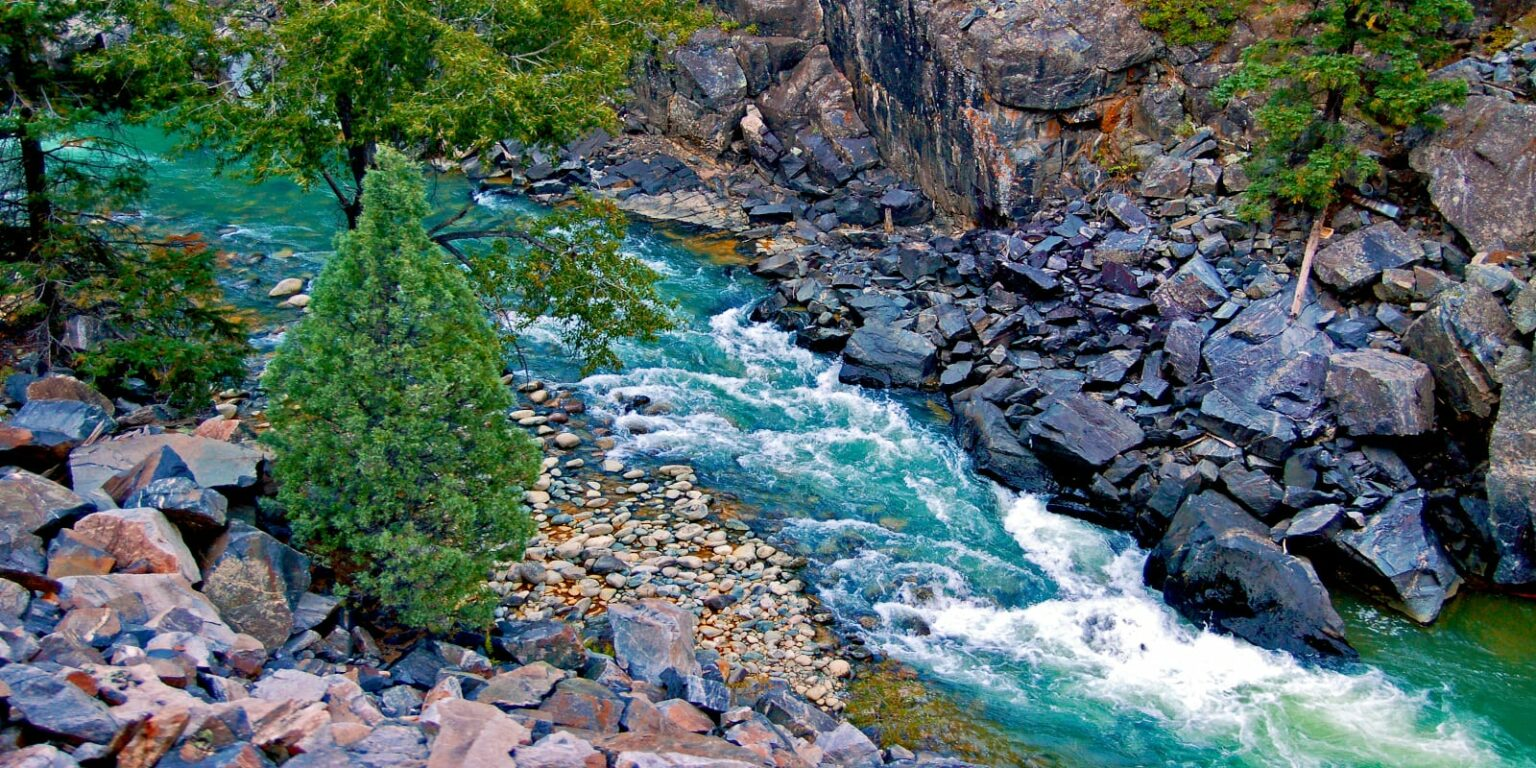
\includegraphics{animas_river.jpg}\\
Snowpack and Discharge:\\
A Case Study on the Animas River}
\usepackage{etoolbox}
\makeatletter
\providecommand{\subtitle}[1]{% add subtitle to \maketitle
  \apptocmd{\@title}{\par {\large #1 \par}}{}{}
}
\makeatother
\subtitle{\url{https://github.com/aislinnmcl/WDAFinalProject}}
\author{Aislinn McLaughlin}
\date{}

\begin{document}
\maketitle

\newpage

\hypertarget{rationale-and-research-questions}{%
\section{Rationale and Research
Questions}\label{rationale-and-research-questions}}

\begin{figure}
\centering
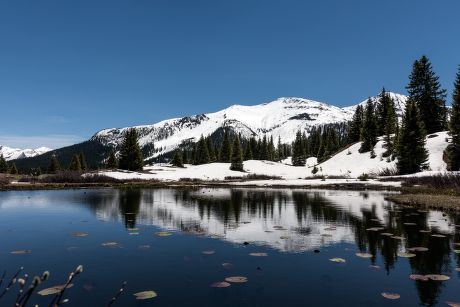
\includegraphics{molas_lake.jpg}
\caption{Molas Lake, Credit: Carol M. Highsmith (2015)}
\end{figure}

While a number of the rivers located in the eastern U.S. have discharge
levels driven primarily by precipitation, many rivers in the western
U.S. are heavily influenced by runoff from snowpack and their discharges
are more seasonal. The relationship between snowpack, measured as
snow-water equivalent (SWE), and discharge is less direct than
precipitation and discharge, and often influenced by a number of other
factors. The author selected this particular region to explore snowpack
and discharge due to her fondness for the area and the time she spent
there in summer 2021.

This project aims to establish a direct relationship between SWE and
discharge through two questions:

\begin{itemize}
\item
  What is the relationship between peak SWE and peak discharge in terms
  of magnitude and timing?
\item
  How has the lag time between peak snowpack and peak discharge changed
  over time?
\end{itemize}

\newpage

\hypertarget{dataset-information-methodology}{%
\section{Dataset Information \&
Methodology}\label{dataset-information-methodology}}

Discharge data was obtained from a USGS gage on the Animas River at
Durango, CO. SWE data was obtained from SNOTEL sensor 632 located at
Molas Lake, approximately 34 miles upstream of the USGS gage. See table
below for more information.

\begin{longtable}[]{@{}lllll@{}}
\toprule
Source & Site & Data.Type & Unit & Range\tabularnewline
\midrule
\endhead
USGS & 09361500 & Discharge & cubic feet per second &
84-10,700\tabularnewline
SNOTEL & 632 & Snow water equivalent & inches & 0-37\tabularnewline
\bottomrule
\end{longtable}

Figure 2 illustrates the location of both data collection sites.
Although the period of record for discharge at this USGS gage extends
from October 1, 1897 to present day, this study is limited to the first
full calendar year of SNOTEL and USGS data. SNOTEL data collection began
at Molas Lake on August 6, 1986. This study examines the period from
1987-2021.

\begin{figure}
\centering
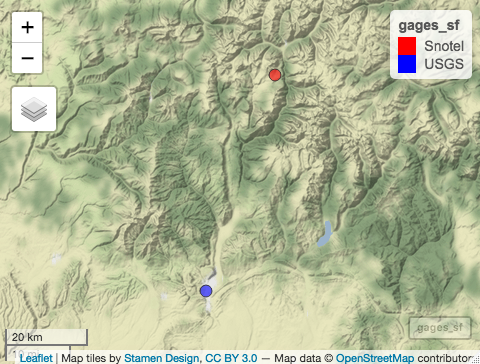
\includegraphics[width=4.5in,height=\textheight]{gage_locations.png}
\caption{Location of the USGS gage on the Animas River at Durango, CO
and the SNOTEL sensor at Molas Lake}
\end{figure}

Peak annual discharge is the maximum daily discharge measured in cubic
feet per second recorded for each year. Peak annual SWE is the maximum
daily SWE measured in inches recorded for each year. To account for
multiple peaks within a calendar year, this study uses the maximum
discharge or maximum SWE recorded at the latest date in each year.

\newpage

\hypertarget{exploratory-analysis}{%
\section{Exploratory Analysis}\label{exploratory-analysis}}

Discharge on the Animas River is very seasonal, typically characterized
by peaks in the months of May and June due to runoff from snowmelt
(Figure 3). A Mann-Kendall test shows that discharge on the Animas has
been decreasing significantly since 1987 (p \textless{} 0.05).

\begin{figure}
\centering
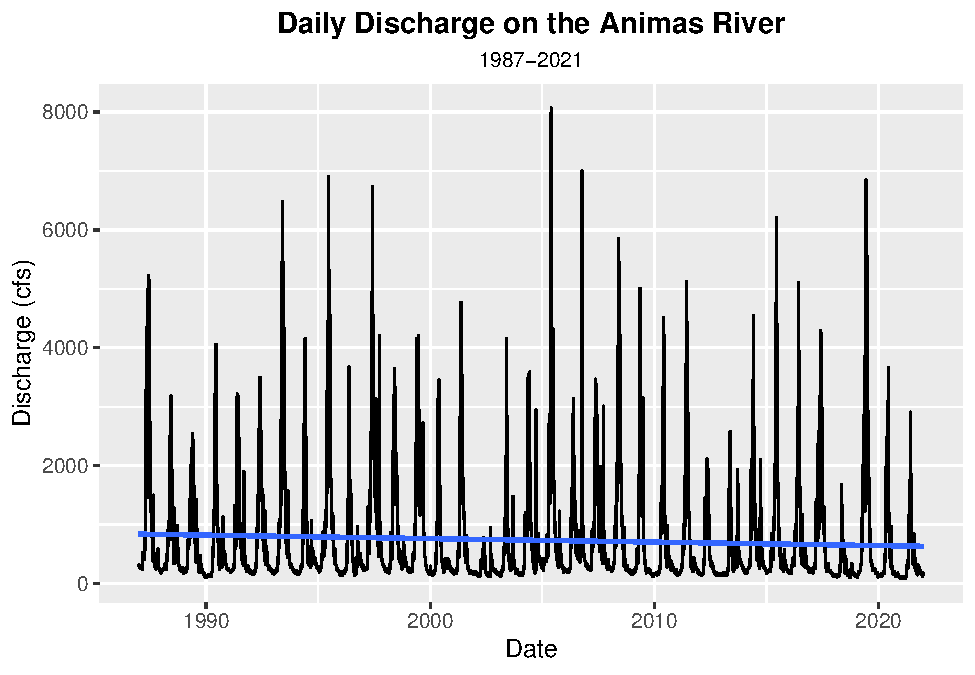
\includegraphics{McLaughlin_WDA_Project_files/figure-latex/unnamed-chunk-2-1.pdf}
\caption{Daily discharge measured in cubic feet per second on the Animas
River at Durango, Colorado}
\end{figure}

\newpage

The seasonality of SWE in the mountains above Durango generally mirrors
that of discharge in the Animas River (Figure 4), although peak SWE
occurs 54 days prior to peak discharge on average. a Mann-Kendall test
reveals that SWE has also been decreasing during the same period. It is
unsurprising that both levels of discharge and SWE have decreased from
1987-2021: a new study reveals that ``2000-2021 was the driest 22-yr
period since at least 800'' (A. Park Williams, 2022).

\begin{figure}
\centering
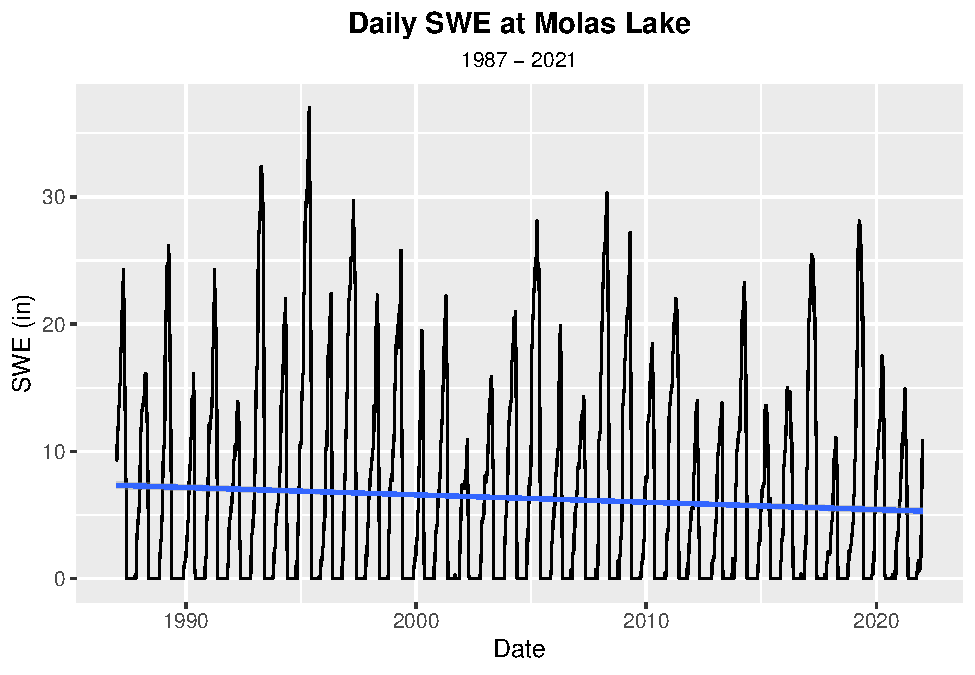
\includegraphics{McLaughlin_WDA_Project_files/figure-latex/unnamed-chunk-3-1.pdf}
\caption{Snow water equivalent at Molas Lake, upstream of the Animas
River USGS gage in Durango}
\end{figure}

\newpage

\hypertarget{analysis}{%
\section{Analysis}\label{analysis}}

\hypertarget{question-1-what-is-the-relationship-between-peak-swe-and-peak-discharge-in-terms-of-magnitude-and-timing}{%
\subsection{Question 1: What is the relationship between peak SWE and
peak discharge in terms of magnitude and
timing?}\label{question-1-what-is-the-relationship-between-peak-swe-and-peak-discharge-in-terms-of-magnitude-and-timing}}

In general, peak SWE and peak discharge appear to mirror each other
quite closely in magnitude (Figure 5). Years with more snowpack
generally also have higher discharges, although the maximum discharges
across the period of record are not necessarily correlated with maximum
SWE. The highest annual maximum discharges on the Animas from 1987-2021
occurred in 2005 and 2006 while the highest annual maximum SWE occurred
in 1995 and 1993.

\begin{figure}
\centering
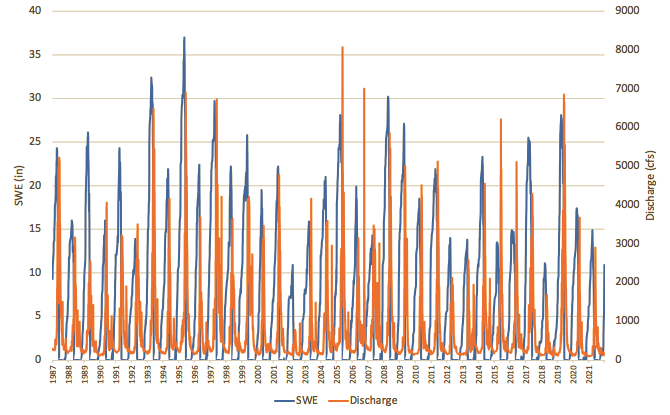
\includegraphics{snowpack_discharge_plot.png}
\caption{SWE-Discharge Relationship}
\end{figure}

A linear model shows that peak SWE explains 43\% of the variability in
peak discharge (p \textless{} 0.001)(Figure 6). Although a linear model
does not show a significant relationship, it also appears that peak SWE
helps determine the day of the year on which maximum annual discharge
occurs: the higher the peak SWE, the more days it takes to reach peak
discharge (Figure 7). A denser snowpack will take longer to melt,
resulting in a delayed peak discharge on the river.

\begin{figure}
\centering
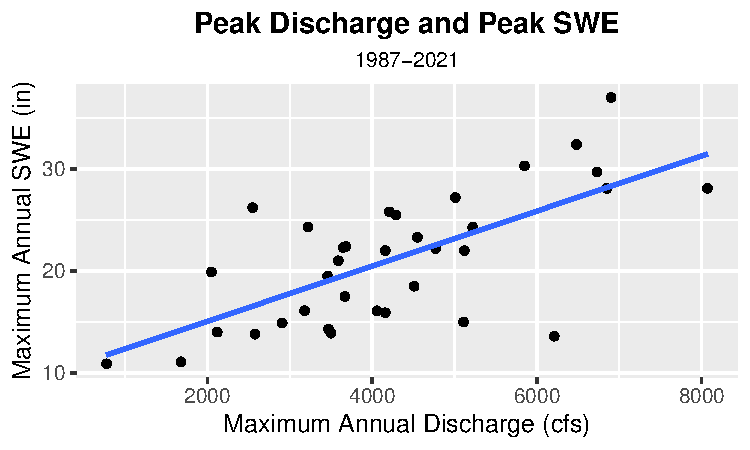
\includegraphics{McLaughlin_WDA_Project_files/figure-latex/unnamed-chunk-5-1.pdf}
\caption{The relationship between peak annual SWE and peak annual
discharge}
\end{figure}

\begin{figure}
\centering
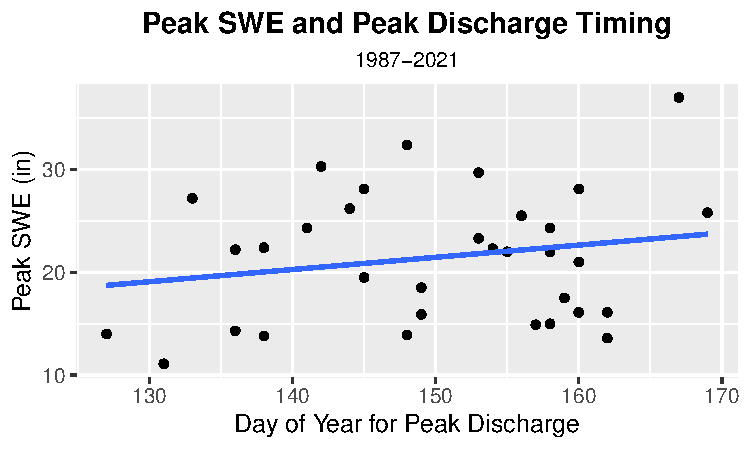
\includegraphics{McLaughlin_WDA_Project_files/figure-latex/unnamed-chunk-6-1.pdf}
\caption{Relationship between peak SWE and the day of the year on which
peak discharge occurs}
\end{figure}

\newpage

\hypertarget{question-2-how-has-the-lag-time-between-peak-snowpack-and-peak-discharge-changed-over-time}{%
\subsection{Question 2: How has the lag time between peak snowpack and
peak discharge changed over
time?}\label{question-2-how-has-the-lag-time-between-peak-snowpack-and-peak-discharge-changed-over-time}}

Although lag time generally seems to be trending upward, a Mann-Kendall
test indicates there is no statistically significant monotonic trend in
lag time from 1987-2021 (p \textgreater{} 0.05) (Figure 8). The
hypothesis that a greater maximum SWE would lead to a longer lag time
was not supported by the analysis which did not reveal any significant
relationship between SWE depth and lag time; in fact, lag time appears
to decrease as peak SWE increases (Figure 9).

\begin{figure}
\centering
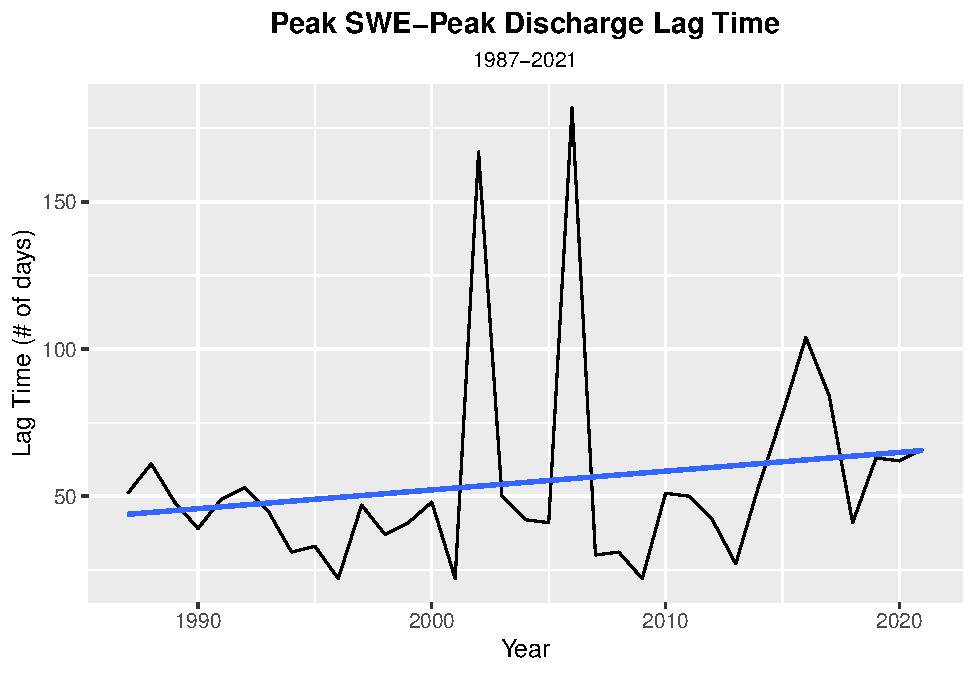
\includegraphics{McLaughlin_WDA_Project_files/figure-latex/unnamed-chunk-7-1.pdf}
\caption{Days between maximum recorded SWE and maximum recorded
discharge for each year from 1987-2021}
\end{figure}

\begin{figure}
\centering
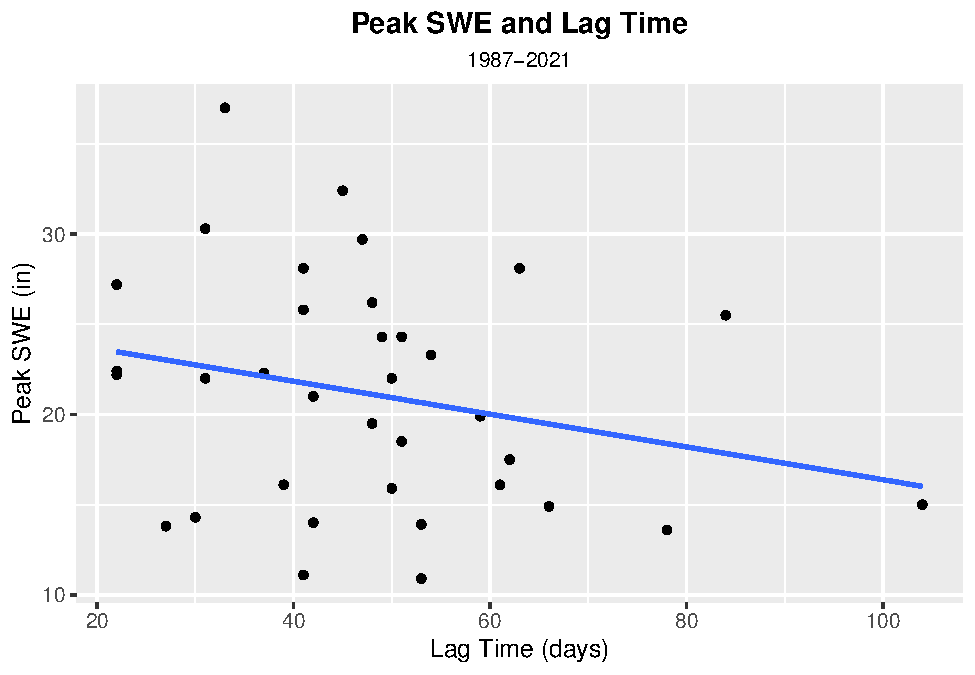
\includegraphics{McLaughlin_WDA_Project_files/figure-latex/unnamed-chunk-8-1.pdf}
\caption{Relationship between peak SWE and lag time to peak discharge}
\end{figure}

\newpage

\hypertarget{summary-and-conclusions}{%
\section{Summary and Conclusions}\label{summary-and-conclusions}}

The results of this study indicate that peak SWE and peak discharge are
directly correlated in terms of magnitude: a higher peak SWE indicates a
higher peak discharge. However, it is more difficult to determine a
significant relationship in terms of timing. There also was not a
significant relationship between peak SWE and lag time: lag time does
not appear to be increasing or decreasing significantly across the
period of record nor does peak SWE seem to determine when during the
year peak discharge occurs.

Several factors outside the scope of this study have a direct impact on
the relationship between SWE and discharge, including soil moisture and
water diversions. If the soil moisture is low at the time the ground
freezes for the winter, then spring runoff from the snowpack must first
rehydrate the soil before flowing down into any other bodies of water.
This would explain why greater peak SWE does not necessarily translate
into greater peak discharge. Additionally, many water rights allocations
exist between the SNOTEL sensor and the USGS stream gage, and many of
those are for irrigation (Figure). Water withdrawals from the Animas
River upstream of the gage would affect the ability to correlate SWE
with discharge.

Although an effort was made to select proximate data sources, the
distance between the SNOTEL sensor and the USGS stream gage could
influence the relationship between SWE and discharge. It is possible
that some of the runoff from snowmelt flowed into a body of water other
than the Animas River or evaporated over the course of its path from
Molas Lake to the Animas.

Future research could focus on constructing a model that incorporates
factors such as soil moisture, precipitation, air temperature, distance
from sensor to gage, local water diversions in addition to SWE and
discharge data. This model would likely provide a much more
comprehensive picture of the relationship between peak SWE and peak
discharge and illustrate the impact of more explanatory variables.

\newpage

\hypertarget{references}{%
\section*{References}\label{references}}
\addcontentsline{toc}{section}{References}

\hypertarget{refs}{}
\begin{CSLReferences}{1}{0}
\leavevmode\hypertarget{ref-WILLIAMS2022232}{}%
A. Park Williams, J. E. S., Benjamin I. Cook. (2022). Rapid
intensification of the emerging southwestern north american megadrought
in 2020--2021. \emph{Nature Climate Change}, \emph{12}, 232--234.
https://doi.org/\url{https://doi.org/10.25921/8pt9-hz08}

\end{CSLReferences}

\end{document}
